% Modelo de Dissertação do Mestrado em Informática da PUC - Alterado para cumprir a normalização de 2011
%\documentclass[a4paper,brazil,ruledheader,normaltoc,capchap]{abnt}

% Para impressão frente e verso (normalização 2011)
\documentclass[a4paper,brazil,ruledheader,normaltoc,capchap,twoside,openany]{abnt_pucmg_utf8}

% Não esquecer das alterações no arquivo abnt.cls
% Se estiver usando o Kile no Ubuntu o arquivo fica armazenado em /usr/share/texmf/tex/latex/abntex.
% Comentar a linha 967 
% \vspace*{30pt}% - Linha comentada para reduzir o espaçamento entre o topo da página e o título \chapter
% Alterar a linha 1143
% \vspace*{-30pt} % - Parâmetro alterado de 30pt para -30pt para reduzir o espaçamento entre o top da página e o título do apêndice
% Alterar a linha 985
%\vspace*{-30pt}\par % - Parâmetro alterado de 0pt para -30pt para reduzir o espaçamento entre o top da página e o título \chapter*
% Alterar a linha 991
% Parâmetro alterado de 45pt para 30pt para reduzir o espaçamento entre o texto e o título \chapter*

% Não esquecer das alterações no arquivo acronym.sty
% Se estiver usando o Kile no Ubuntu o arquivo fica armazenado em /usr/share/texmf-texlive/tex/latex/acronym
% Alterar a linha 225
%\item[\protect\AC@hypertarget{#1}{\acsfont{\normalfont{#2}}} --] #3% - Inserir separador entre acrônimo/descrição e remover o negrito com o normalfont

% Pacote para definir explicitamente as margens das páginas
\usepackage[a4paper,left=3cm,right=2cm,top=3cm,bottom=2cm]{geometry}

%\usepackage{units}
% Utilize da seguinte forma \unit[78,6]{mA}

% Pacote para gerenciar siglas
\usepackage[printonlyused]{acronym}

% Merge em duas células (linhas diferentes)
\usepackage{multirow}

% Pacote para citação e referências seguindo ABNT no sistema (AUTOR, Data)
%\usepackage[alf, bibjustif,abnt-emphasize=bf]{abntcite}
%\usepackage[alf, abnt-emphasize=em, abnt-thesis-year=title]{abntcite}
\usepackage [alf]{abntcite}
% @article An article from a journal or magazine 
% @inproceedings An article in a conference proceedings
% Força que o tipo de ênfase no nome do simpósio seja em caixa alta
\renewcommand{\emph}{\textsc}

% Pacote para múltiplos arquivos .bib
\usepackage{multibib}
%\newcites{pub}{Refer\^encias das publica\c{c}\~oes}

% Pacotes de codificação das fontes para português
\usepackage[brazil]{babel}

% Pacote para citação e referências seguindo ABNT no sistema (AUTOR, Data)
%\usepackage[alf, bibjustif,abnt-emphasize=bf]{abntcite}
%\usepackage[alf, abnt-emphasize=em, abnt-thesis-year=title]{abntcite}
% @article An article from a journal or magazine 
% @inproceedings An article in a conference proceedings
% Força que o tipo de ênfase no nome do simpósio seja em caixa alta
%\renewcommand{\emph}{\textsc}


% Pacote de adequação do formato ABNT para normas da PUCMinas
\usepackage{abnt-PPGInf-PUCMG}

% Pacotes utilitários
\usepackage{graphicx}

% Pacote para fixar a figura no local desejado
\usepackage{float}

% Pacote para adicionar simbolos as informações de rodapé
\usepackage[symbol]{footmisc}

\usepackage[all]{xy}
%\usepackage[tight]{subfigure}	% Permite a criação de subfiguras
\usepackage{url,amsmath}	% Permite melhorias na codificação de fórmulas
%\usepackage{amsthm}		% Permite melhorias na escrita de teoremas
\usepackage{amssymb}		% Permite utlização de simbolos matemáticos avançados

\usepackage[portuguese, linesnumbered, ruled, vlined]{algorithm2e}
\usepackage{algorithmic} 	% para algoritmos
\usepackage{listings} 		% para importação de código-fonte

% Alterar o espaçamento da margem no algoritmo
\setlength{\algomargin}{1em}

\usepackage{setspace}

% Pacote para rotação de tabelas/figuras
\usepackage{rotating}

% Pacotes para criação de cronograma/tabela colorida
\usepackage{color}
\usepackage{array}
\usepackage{longtable}
\usepackage{colortbl}
%\definecolor{lightgray}{gray}{0.9}

% Pacote para possibilitar o uso do setboolean para forçar formatos de página diferentes do padrão do documento
\usepackage{ifthen}

% Para inserir captions (nova normalização 2011)
\usepackage[size=normalsize,labelfont=bf,textfont={bf},labelsep=endash]{caption}
\captionsetup[subfloat]{labelfont=bf,textfont={bf}}

% Usado para reduzir espaçamentos entre itens (alíneas, enumerações) com o compactitem
\usepackage{paralist}

% Alterar para sequencial a numeração de figuras e tabelas
\captionsetup{figurewithin=none}
\captionsetup{tablewithin=none}

\setlength{\LTcapwidth}{\textwidth}

% Para o subsubsection aparecer no sumário 
\setcounter{tocdepth}{3}
\setcounter{secnumdepth}{3}

% Para inserir referências via links - não funciona para abntex
%\usepackage[colorlinks=true,pdfstartview=FitV,linkcolor=blue,citecolor=blue,urlcolor=blue,hyperindex,pagebackref=true,pdftex,breaklinks]{hyperref}
%\usepackage[pdftex]{hyperref}

% Para criar lista de gráficos
\floatstyle{plaintop}
\newfloat{grafico}{H}{loq}
\restylefloat*{grafico}
\floatname{grafico}{Gráfico} 

% Para gerar subfiguras usando o subfloat
\usepackage{subfig}
\newsubfloat[position=bottom,listofformat=subsimple]{grafico}

% define estilo de posicionamento na caixa
\newsavebox{\leftfig}
\newsavebox{\rightfig}

%\renewcommand{\ALG@name}{Algoritmo}
%\renewcommand{\listalgorithmname}{Lista de Algoritmos}

% Configuração de código-fonte
\lstset{extendedchars=\true, % permite acentos
 inputencoding=utf8,
 literate={\$}{{\$}}1,
 commentstyle=\it, % deixa os comentários em itálico
 stringstyle=\bf, % não lembro o que faz, mas está funcionando
 belowcaptionskip=5pt, % não lembro o que faz, mas está funcionando
 numbers=left, % coloca a numeração na esquerda
 stepnumber=1, % passos da numeração
 firstnumber=1, % primeira linha
 numberstyle=\tiny, % tamanho da fonte da numeração
 breaklines=true, % permitir quebra de linha
 frame=tb, % borda em cima e em baixo
 basicstyle=\footnotesize, % estilo básico
 stringstyle=\ttfamily, % não lembro o que faz, mas está funcionando
 showstringspaces=false, % não mostrar os espaços
 mathescape, % não lembro o que faz, mas está funcionando
 tabsize=3 % tamanho da tabulação
}
\renewcommand{\lstlistingname}{Código}
\renewcommand{\lstlistlistingname}{Lista de Códigos}
\citeoption{abnt-etal-cite=1, abnt-and-type=e}

% the bibtex style generates this command, but it's not defined

%%\pdfinfo{%
%%  /Title    (TITULO DA DISSERTACAO)
%%  /Author   (Nome do aluno)
%%  /Creator  (Nome do aluno)
%%  /Producer (Kile - an Integrated LaTeX Environment - %%Version 2.0.85)
%%  /Subject  (Dissertação de Mestrado)
%% /Keywords (Palavras chave)
%%}

% PRÉ-TEXTUAIS %%
\begin{document}

% Para forçar que elementos pré-textuais (da capa até o sumário) sejam impressos no anverso da folha
\setboolean{@twoside}{false}

\autor{Bergson Monteiro da Silva Junior}

% Coloque o título em caixa alta. É o padrão da PUC.
% Vá no arquivo abnt-PPGInf-PUCMG.sty e procure por esse título (linha 575). Altere para o seu título em caixa alta. Isso será utilizado na folha de aprovação.
\titulo{Desenvolvimento de aplicativo multiplataforma para controle de empréstimos em laboratório}

\orientador[Orientadora: ]{Profa. Michelle Nery Nascimento}

% Se não tiver, co-orientador, comente a próxima linha.
%\coorientador[Co-orientador:]{Professor}

% Texto
%\comentario{Dissertação apresentada ao Programa de Pós-Graduação em Informática da Pontifícia Universidade Católica de Minas Gerais,
%como requisito parcial para obtenção do título de Mestre em Informática.}


% Instituição
%\instituicao{Mestrado em Informática \par Instituto de Informática \par Pontifícia Universidade Católica de Minas Gerais}

% Local
\local{Belo Horizonte}

% Data
\data{}
\capa
%Para forçar que a ficha catalográfica seja impressa no verso da folha de aprovação
\setboolean{@twoside}{true}

% Gera a folha de rosto
\folhaderosto

% Ficha catalográfica
%% Ficha catalográfica
% INCLUIR O ARQUIVO PDF GERADO PELA BIBLIOTECA COMO FIGURA.
\begin{figure}[h!]
	\vspace*{-3.3cm}
	\hspace*{-3cm}
%	% Suponha o nome do arquivo em pre-texto/ficha-catalografica/fichacatalografica.pdf
	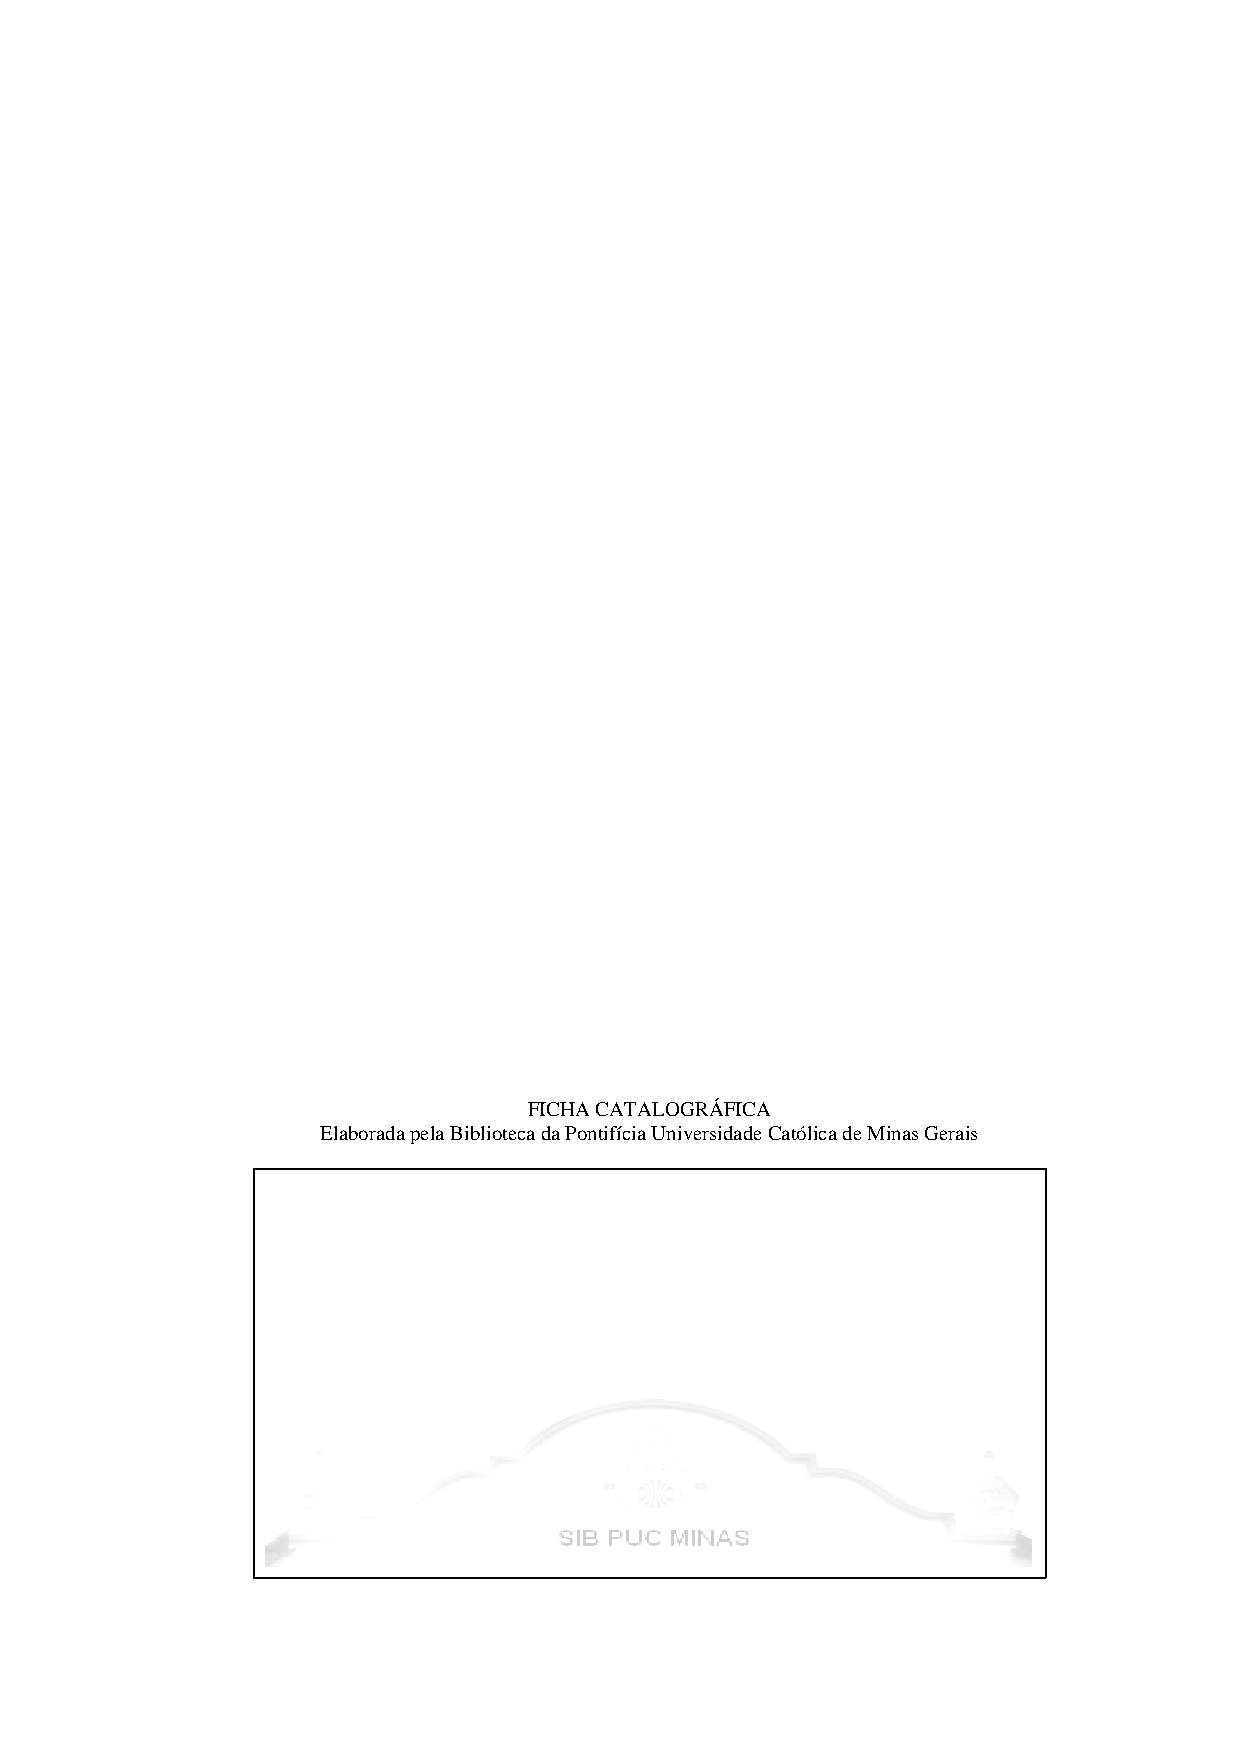
\includegraphics{pre-texto/ficha-catalografica} 
	\newpage
\end{figure}

% Para forçar que elementos pré-textuais (da capa até o sumário) sejam impressos no anverso da folha
\setboolean{@twoside}{false}

% Folha de aprovação
%% Termo de Aprovação

% Texto da aprovação
\textoaprovacao{Dissertacao apresentada ao Programa de Pos-Graduacao em Informatica como requisito parcial para qualificacao ao Grau de Mestre em Informatica pela Pontificia Universidade Catolica de Minas Gerais.}

% Primeira assinatura
\primeiroassina{Prof. Dr. Orientador -- PUC Minas}

% Segunda assinatura
\segundoassina{Prof.$^{a}$ Dr.$^{a}$ Membro interno -- Instituicao}

% Terceira assinatura
\terceiroassina{Prof. Dr. Membro externo -- Instituicao}

% Quarta assinatura
%\quartoassina{}

% Data da defesa
\localdia{Belo Horizonte, data da defesa.}

% Gera o termo de aprovação
\termodeaprovacao	

% Dedicatória
%% Dedicatória
\newpage

% Espaçamento do topo da página até o texto da dedicatória
\vspace*{22cm}

% Espaçamento na esqueda
\hspace{8cm}\begin{minipage}{.60\textwidth}
            \textit{texto de dedicatoria}
            \end{minipage}

% Agradecimentos
%% Agradecimentos
%\chapter*{Agradecimentos}
\begin{center}
	\normalsize
	\textbf{AGRADECIMENTOS}
	
	texto
\end{center}

 

% Epígrafe
%% Epígrafe
\newpage

% Espaçamento entre topo da página e texto da epígrafe
\vspace*{10cm}
% Espaçamento na esqueda
\hspace{4cm}\begin{minipage}{.51\textwidth}

% Texto da epígrafe
\textit{``E fazendo que se aprende a fazer aquilo que se deve aprender a fazer.'' }

%Nome do autor
\begin{flushright}\itshape Aristoteles \upshape\end{flushright}

\end{minipage}

% Resumo
% Resumo
\begin{resumo}
% Diminuir espaçamento entre título e texto
\vspace{-1cm}

% Texto do resumo: sem paragrafo, justificado, com espaçamento 1,5 cm
\onehalfspacing

\noindent 
  Com o avanço tecnológico cada vez mais presentes no cotidiano das pessoas, a informatização de processos manuais se faz mais necessário em algumas organizações. Portanto, este trabalho tem como objetivo criar um aplicativo de \textit{smartphone}, que realiza empréstimos dos equipamentos do laboratório de fotografia e áudio visual da PUC Minas, facilitando o processo de empréstimo e o tornando mais ágil e eficiente. Para o desenvolvimento do aplicativo, foi utilizado uma tecnologia multiplataformas, permitindo a construção de um único código para diversas plataformas \textit{mobile}. O trabalho apresenta conceitos e características do desenvolvimento \textit{mobile}, tais como vantagens, desvantagens, peculiaridades, dentre outros pontos importantes para alcançar o objetivo geral do trabalho. A construção da aplicação deu se por etapas, partindo de um entendimento geral do escopo e as necessidades dos envolvidos junto a análise de requisitos para definir quais as funcionalidades deveriam ser implementas, definição da arquitetura e prototipagem do aplicativo, em seguida o desenvolvimento, testes e o processo de homologação para validar a implementação das funcionalidades e simular o funcionamento da aplicação em ambiente real.

% Espaçamento para as palavras-chave
\vspace*{.75cm}

% Palavras-chave: sem parágrafo, alinhado à esquerda
\noindent Palavras-chave: Mobile, Desenvolvimento, React Native, Multiplataforma
% Segunda linha de palavras-chave, com espaçamento.
%\indent\hspace{2cm}Palavra.

\end{resumo}

% Abstract
%% Abstract
\begin{abstract}
% Diminuir espaçamento entre título e texto
\vspace{-1cm}
% Texto do resumo, em inglês: sem paragrafo, justificado, com espaçamento 1,5 cm
\onehalfspacing
\noindent
  Texto do resumo, em ingles.

% Espaçamento para as palavras-chave
\vspace*{.75cm}

% Palavras-chave: sem parágrafo, alinhado à esquerda
\noindent Keywords: . \\
% Segunda linha de palavras-chave, com espaçamento.
%\indent\hspace{1.4cm} Keyword.

\end{abstract}

\makeatletter
\renewcommand\numberline[1]{
	\leftskip 0em
	\rightskip 1.6em
	\parfillskip -\rightskip
	\parindent 0em
	\@tempdima 2.0em
	\vspace{0em} \advance\leftskip \@tempdima \null\nobreak\hskip -\leftskip
	FIGURA \normalfont #1 -- }
\makeatother

% Lista de figuras
\listoffigures

\makeatletter
\renewcommand\numberline[1]{
	\leftskip 0em
	\rightskip 1.6em
	\parfillskip -\rightskip
	\parindent 0em
	\@tempdima 2.0em
	\vspace{0em} \advance\leftskip \@tempdima \null\nobreak\hskip -\leftskip
	TABELA \normalfont #1 -- }
\makeatother

% Lista de tabelas
\listoftables

\makeatletter
\renewcommand\numberline[1]{
	\leftskip 0em
	\rightskip 1.6em
	\parfillskip -\rightskip
	\parindent 0em
	\@tempdima 2.0em
	\vspace{0.5em} \advance\leftskip \@tempdima \null\nobreak\hskip -\leftskip
	GRÁFICO \normalfont #1 -- }
\makeatother

% Lista de graficos
%\listof{grafico}{Lista de Graficos}

% Lista de siglas
%% Lista de Abreviaturas e Siglas
%\chapter*{Lista de Abreviaturas e Siglas}
\chapter*{Lista de Abreviaturas e Siglas}

% Mantenha sempre em ordem alfabética.

\begin{acronym}
\acro{BER} {\textit{Bit Error Rate}}
\acro{BT} {\textit{Block Tri-diagonal}}
\acro{CG} {\textit{Conjugate Gradient}}
\acro{CSS} {\textit{Chirp Spread Spectrum}}
\acro{DCC-MAC} {\textit{Dynamic Channel Coding} MAC}
\acro{DSSS} {\textit{Direct-sequence spread spectrum}}
\acro{EP} {\textit{Embarrassingly Parallel}}
\acro{FIFO} {\textit{First In, First Out}}
\acro{FT} {\textit{Fast Fourier Transform}}
\acro{IEEE} {\textit{Institute of Electrical and Electronics Engineers}}
\acro{IR-UWB} {\textit{Impulse Radio} UWB}
\acro{IS} {\textit{Integer Sort}}
\acro{LU} {\textit{Lower-Upper Gauss-Seidel}}
\acro{MAC} {\textit{Medium Access Control}}
\acro{MB-OFDM} {\textit{Multi-Band Orthogonal Frequency Division Multiplexing}}
\acro{MG} {\textit{Multi-Grid}}
\acro{MPE} {MPI \textit{Parallel Environment}}
\acro{MPI} {Interface de passagem de mensagem, do inglês \textit{Message Passing Interface}}
\acro{NAS} {NASA \textit{Advanced Supercomputing}}
\acro{NOAH} {\textit{No Ad-Hoc Routing Agent}} 
\acro{NS-2} {\textit{Network Simulator} 2}
\acro{NoCs} {Redes-em-Chip, do inglês \textit{Networks-on-Chip}}
\acro{NPB} {NAS \textit{Parallel Benchmark}}
\acro{OpenMP} {Multi-processamento aberto, do inglês \textit{Open Multi-Processing}}
\acro{PHY} {\textit{Physical Layer}}
\acro{PPM} {\textit{Pulse-Position Modulation}}
\acro{SP} {\textit{Scalar Penta-diagonal}}
\acro{TH} {\textit{Time Hopping}}
\acro{THS} {\textit{Time Hopping Sequence}}
\acro{UDP}{\textit{User Datagram Protocol}}
\acro{UWB} {\textit{Ultra Wide Band}}
\acro{WiNoCs} {Redes-em-Chip Sem Fio, do inglês \textit{Wireless Networks-on-Chip}}
\acro{WLAN} {Rede Local Sem Fio, do inglês \textit{Wireless Local Area Network}}
\acro{WPAN} {Rede de Área Pessoal Sem Fio, do inglês \textit{Wireless Personal Area Network}}
\end{acronym}

\makeatletter
\renewcommand\numberline[1]{#1\hspace{0.8em}}
\makeatother

% Altera para espaçamento simples a partir daqui
\singlespacing

% Sumário
\tableofcontents

% Altera para espaçamento 1,5 a partir daqui
\onehalfspacing

%% TEXTUAIS 
% Para forçar que elementos textuais e pós-textuais sejam impressos no anverso e verso das folhas
\setboolean{@twoside}{true}
% Altere o número da página para o correto. Conte todas as páginas frente e verso, menos a capa, nclusive a ficha catalográfica até a página do primeiro capítulo.
\setcounter{page}{25}

% Capítulos
% Para forçar que o capítulo de introdução comece no anverso
\setboolean{@openright}{true}
% Nome do capítulo
\chapter{Introdução}
% Label para referenciar
\label{cap1}

% Diminuir espaçamento entre título e texto
\vspace{-1.9cm}

% Texto do capítulo

    Uma aplicação móvel é um software projetado para ser executado em \textit{smartphones, tablets} ou outros dispositivos móveis e podem ser classificados em três categorias, sendo nativos, híbridos ou nativos multiplataformas. Conforme estudo realizado pela empresa de consultoria App Annie, o uso destas aplicações para realizar tarefas diárias cresce cada vez mais, principalmente no Brasil, que se encontra em terceiro lugar no \textit{ranking} mundial \cite{AppAnnie2020}.

    O desenvolvimento de aplicações nativas consiste na construção de aplicações dedicadas e projetadas somente a um sistema operacional,  pelo fato de cada plataforma possuir compatibilidade nativa com determinadas linguagens de programação, por exemplo o \textit{Swift} para iOS e o \textit{Kotlin} para Android. Todas as funcionalidades da plataforma estão disponíveis sem restrições e existem padrões de interface gráfica e experiência de usuário específicos, que ajudam o usuário a entender como aquele aplicativo funciona, já que todos os outros aplicativos daquela plataforma seguem os mesmos padrões \cite{Corral2012}.
    
    Além das aplicações nativas, existem também as \textit{Web Apps(PWAs)} que são aplicações web híbridas podendo ser executadas no \textit{browser} de cada dispositivo. O desenvolvimento destas aplicações é baseado em linguagens como HTML, CSS e \textit{Javascript} para o \textit{client-side} e para o \textit{server-side} pode-se utilizar \textit{Ruby}, \textit{Java}, PHP entre outras. Com as \textit{Web Apps} é possível desenvolver uma mesma aplicação a ser executada em dispositivos de diferentes plataformas, porém não é possível ter acesso total às funcionalidades de cada plataforma, como no desenvolvimento nativo, e também não existem padrões de interface ou de experiência de usuário que sirva para várias plataformas ao mesmo tempo, podendo causar uma sensação ruim na usabilidade e experiência de uso da aplicação \cite{Corral2012}.

    A abordagem nativa multiplataformas no desenvolvimento \textit{mobile} diz respeito à criação de uma aplicação através de um único processo de desenvolvimento, onde o resultado final é um aplicativo instalável e executável em diferentes sistemas operacionais, como iOS e Android. Segundo \protect\cite{SantosMontan2012}, nos últimos anos, o esforço gasto para o desenvolvimento nativo proporcionou o surgimento de alternativas comerciais, como os \textit{frameworks} para desenvolvimento multiplataforma \textit{(Cross Platform)} como \textit{Flutter}, \textit{React Native} e \textit{Xamarin}, ganharam espaço no mercado tecnológico por esta abordagem híbrida, pelo fato de acelerar o processo de desenvolvimento, permitindo a criação de aplicativos para diferentes plataformas a partir de um mesmo código, o que impacta diretamente no custo de um projeto, dado que menos recursos técnicos serão necessários para a sua conclusão \cite{Barguil2019}. O \textit{React Native}, criado em 2015 pelo Facebook, é um \textit{framework} referência no desenvolvimento nativo multiplataformas, proporcionando ferramentas e padrões para um desenvolvimento ágil e de qualidade, garantindo um desempenho, performance e usabilidade similar ao de aplicações exclusivamente nativas entre outros recursos que são explicitados ao longo desta dissertação. Antes do seu surgimento o desenvolvimento nativo era algo mais complexo, pois era necessário ter o conhecimento de linguagens específicas como \textit{Swift} para o desenvolvimento de aplicações em iOS e \textit{Java}, \textit{Kotlin} e C++ para Android, impossibilitando qualquer reaproveitamento de código e requisitando equipes de trabalho com o conhecimento em várias tecnologias \cite{Charland2011}.
  
    Com o grande avanço da tecnologia móvel, a informatização de processos manuais utilizando as tecnologias citadas anteriormente vem se tornando cada vez mais presente e necessário no contexto de determinadas organizações que visam adquirir maior agilidade e praticidade na execução, disponibilidade e integridade das informações pertinentes durante seus processos, de maneira interativa que garanta uma experiência fluída ao usuário. Trazendo um exemplo real, no laboratório de áudio visual e fotografia da PUC Minas unidade São Gabriel existe uma dificuldade, como também ineficiência e falta de agilidade para realizar a gestão e controle de empréstimos dos equipamentos. Atualmente, os alunos da universidade entram em contato com monitores e técnicos do laboratório para verificar a disponibilidade de um determinado equipamento e, caso o equipamento esteja disponível, o aluno preenche um formulário disponibilizado pelo próprio laboratório para manter o controle dos recursos. Após o preenchimento deste formulário, o monitor ou técnico preenche uma planilha com dados do equipamento para atualizar sobre a situação de empréstimo do mesmo. Em seguida, a liberação é feita por este responsável que conduziu o processo. Em muitos casos a consulta sobre a disponibilidade de determinado recurso é lenta devido à presença de algum dado inconsistente na planilha de controle dos equipamentos, além do que algumas destas informações se perdem durante o processo, sendo que não há uma base de dados centralizada para armazenar todas as informações que auxiliam na gestão e no controle dos recursos do laboratório.
    
    Dado o contexto, este trabalho de conclusão de curso tem como principal objetivo desenvolver uma aplicação \textit{mobile} utilizando \textit{React Native}, com funcionalidades que auxiliem na agilidade e praticidade dos empréstimos do laboratório e com regras de negócios que garantam a disponibilidade, integridade e persistência dos dados. Desta maneira, a aplicação a ser desenvolvida poderá ser utilizada por monitores e técnicos do laboratório, alunos e professores da PUC Minas.


\section{Objetivos}
\label{secao1}

    Esta seção apresenta os objetivos gerais e específicos definidos para este trabalho.

\subsection{Objetivo Geral}
  
    Este trabalho tem por objetivo desenvolver uma aplicação \textit{mobile} multiplataformas que irá suportar de maneira informatizada o processo de empréstimos de equipamentos dos laboratórios de audiovisual e fotografia da PUC Minas visando centralizar os dados e informações importantes ao processo de maneira simplificada e objetiva, assegurando uma experiência fluída aos usuários.
    
\subsection{Objetivos Específicos}
  
  Os objetivos específicos deste trabalho são:

    \begin{compactitem}
      \item[a)] Elicitar todos os requisitos arquiteturais e prototipar a aplicação;
      \item[b)] Desenvolver uma aplicação \textit{mobile} em \textit{React Native}, para iOS e Android, com funcionalidades que auxiliem a agilidade e praticidade dos empréstimos;
      \item[c)] Definir regras de negócio e estratégias de persistência a dados para garantir a disponibilidade, confiabilidade e integridade das informações do fluxo de empréstimo;
      \item[d)] Disponibilizar o aplicativo a monitores, técnicos, alunos e professores da Universidade;
      \item[e)] Facilitar a consulta sobre a disponibilidade dos equipamentos do laboratório.
    \end{compactitem}

\section{Justificativa}

    O crescimento do mercado \textit{mobile} deixou de ser uma tendência e passou a ser uma realidade em todos os lugares do mundo, com isso as empresas podem explorar este potencial tecnológico para se diferenciarem de seus concorrentes, otimizando e/ou automatizando processos internos ou externos, aprimorando a gestão organizacional e também agregando valor ao seu negócio. Estes são alguns pontos que o desenvolvimento deste trabalho atingirá diretamente no contexto organizacional em que poderá ser aplicado, como também no cotidiano dos colaboradores e alunos que participam do processo de empréstimo dos equipamentos do laboratório de audiovisual e fotografia da PUC Minas; dado que as tecnologias \textit{mobile} viabilizam uma interação rica e intuitiva, principalmente com telas \textit{touch screen}, onde abre novas maneiras para usuários e desenvolvedores permitindo experiências totalmente novas onde não seria possível sem a tecnologia \textit{mobile} \cite{SousaMonteiro2015}.
    
    Além das vantagens citadas no paragráfo anterior, o desenvolvimento deste trabalho pode gerar os seguintes benefícios:
    
     - Agilidade no processo de empréstimo de equipamentos;
     
     - Auxiliar no controle dos equipamentos, visando a disponibilidade, prazos de devolução, datas de empréstimo e responsáveis pelos empréstimos;
     
     - Informações centralizadas para facilitar a gestão dos empréstimos aos alunos.
% Os demais capítulos não precisam começar no anverso
\setboolean{@openright}{false}
% Nome do capítulo
\chapter{Referencial Teórico}
% Label para referenciar
\label{cap2}

% Diminuir espaçamento entre título e texto
\vspace{-1.9cm}

% Texto do capítulo

    Nesta seção são abordados alguns conceitos e definições importantes para a compreensão do desenvolvimento de aplicações híbridas, alguns componentes que fazem parte do ecossistema mobile e os principais desafios enfrentados por essas tecnologias.
  
\section{A tecnologia \textit{mobile}}

    Assim como em computadores, os dispositivos móveis também possuem diversas opções de sistemas operacionais, dentre elas, os principais são iOS desenvolvido pela \textit{Apple} e Android pelo \textit{Google}. 

    Com a criação dos \textit{smartphones} e \textit{tablets} e a grande quantidade de inovações que estes dispositivos trouxeram junto aos seus sistemas operacionais, os consumidores deixaram de utilizar estes dispositivos somente para ligações ou simples trocas de mensagens, devido a isso, muitas empresas passaram a utilizar deste meio e adaptaram suas necessidades de negócio para gerar conteúdos que atraiam seus clientes, além de prestar serviços de atendimento de maneira rápida e objetiva.
    
    Segundo \citeonline{Galvao2019} esse comportamento do uso do \textit{mobile} é mais do que uma tendência: é uma realidade. Posto que algumas organizações já adaptaram seus processos externos, visando um melhor relacionamento com seus clientes, algumas empresas também tendem a utilizar estas tecnologias visando o ambiente interno. Atualmente, é bastante comum serem usados aplicativos corporativos com foco na otimização de processos e no aperfeiçoamento da comunicação interna \cite{Finzi2019}. A melhoria de processos internos em empresas se faz mais presente no cotidiano das organizações com o avanço do mercado tecnológico e a série de benefícios que estas melhorias podem gerar.

    \subsection{iOS e Android}
      \label{iOS&Android}
      
      Nos últimos anos, o mercado de smartphones tem testemunhado uma batalha entre dois gigantes da tecnologia, a saber, \textit{Apple} e \textit{Google}, empresas responsáveis pelos sistemas operacionais iOS e Android, respectivamente \cite{Cezar2018}. As subseções \ref{iOS} e \ref{Android} apresenta de forma objetiva os principais aspectos de cada sistema operacional afim de contextualizar sobre a representatividade de cada um no meio tecnológico.
      
      \subsubsection{iOS}
       \label{iOS}
       
       O iOS, abreviatura para o nome \textit{iPhone Operation System} é o sistema operacional desenvolvido e mantido pela \textit{Apple}. Em meados de 2007 Steve Jobs apresentou para o mundo o primeiro dispositivo móvel com o sistema iOS, e teve como uma de suas principais características não permitir que o sistema fosse executado em hardware de terceiros, isto é, ele é encontrado somente em aparelhos da própria marca \cite{SARTORELI2018}.
       
       Atualmente, a \textit{Apple} libera versões de atualização geral de seu sistema uma vez por ano, junto ao lançamento de novos dispositivos eletrônicos em grandes eventos organizados pela empresa, são datas esperadas por muitos dos consumidores dos produtos \textit{Apple}, afim de conhecerem os novos produtos e as inovações implementadas no sistema.
      
      \subsubsection{Android}
       \label{Android}
      
      É uma plataforma para tecnologia móvel baseada em uma versão modificada do núcleo \textit{Linux} e de outros \textit{softwares} \textit{open-source}, idealizada por um consórcio de desenvolvedores conhecido como \textit{Open Handset Alliance}(OHA), atualmente o sistema operacional é mantido pelo \textit{Google} no objetivo em conceder uma resposta à crescente demanda da tecnologia móvel no mundo. O Android foi construído com a intenção de permitir aos desenvolvedores criar aplicações móveis que possam tirar total proveito do que um aparelho portátil possa oferecer \cite{pereiraandroid}.
      
      Criado em 2003 pela Android Inc., e vendido ao \textit{Google} em 2005 o que marcou o surgimento do \textit{Google Mobile Division} que fora o primeiro passo para o início da jornada do \textit{Google} no mercado de dispositivos móveis, dois anos depois o Android foi revelado e no ano seguinte lançaram o primeiro dispositivo Android. Na época atual, o Android está presente em grande parte dos recursos inteligentes, como \textit{Smart TV's}, \textit{SmartWatches}, diversos fabricantes de \textit{smartphones} e \textit{tablets}, variantes do Android estão presentes também em \textit{joysticks}, câmeras digitais, computadores entre outros, isso fez com que este sistema se tornasse o mais utilizado em todo o mundo.
      
  \section{Aplicações \textit{mobile}}

  Além das aplicações nativas multiplataformas que são o foco deste trabalho também serão demonstradas as aplicações nativas e híbridas, para que se possa observar as principais diferenças entre as mesmas e identificar em quais contextos melhor se adequa cada tipo de aplicação.

    \subsection{Aplicações nativas}
      \label{app_nativas}
  
    Aplicativos nativos representam uma forma tradicional e comum de desenvolver para dispositivos móveis. Desenvolver uma aplicação nativa exige a prévia definição de um sistema operacional no qual a aplicação poderá ser instalada e executada.
    
    Por ser desenvolvido exclusivamente a um sistema operacional, o código destas aplicações não pode ser reaproveitado no intuito de desenvolver a mesma aplicação para um outro sistema, tornando o desenvolvimento destas aplicações mais custoso, requisitando equipes específicas que dominam a tecnologia a ser utilizada. 
    
    \begin{figure}[h]
    \caption{Ciclo de desenvolvimento de aplicativos nativos}
    \centering % para centralizarmos a figura
    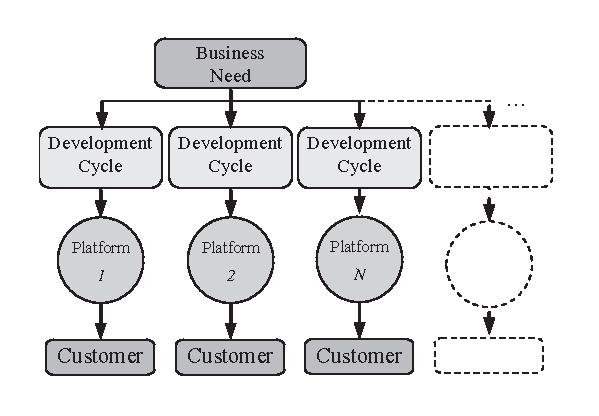
\includegraphics[width=10cm]{imagem/native-development.png}
    \caption*{Fonte: \cite{Corral2012}}
    \label{figura:native-development}
    \end{figure}
    
    Conforme apresentado na figura \ref{figura:native-development}, partindo de uma mesma necessidade de negócio da organização são gerados diferentes ciclos de desenvolvimento com diferentes tecnologias e linguagens para cada plataforma em que o aplicativo poderá ser executado. No Android, por exemplo, é possível utilizar \textit{Java}, \textit{Kotlin} ou C++, no iOS utiliza-se o \textit{Objective-C} ou \textit{Swift} como linguagem de programação.
    
    Existem diversos fatores positivos no desenvolvimento de aplicações nativas. Dado que as aplicações são desenvolvidas exclusivamente para cada ambiente, segue-se os padrões e normas técnicas, de interface e de experiência de usuário determinados pelo sistema, fornecendo uma melhor sensação de aplicação nativa aos usuários. Aplicações nativas têm fácil acesso, por meio de APIs fornecidas pelas plataformas, a recursos dos dispositivos móveis, como sensores, câmera, GPS, contatos e e-mail \cite{S.ElKassas2015}.
    
    \subsection{Aplicações híbridas}
        \label{app_hibridas}
    
    Apesar das vantagens citadas na subseção \ref{app_nativas}, o desenvolvimento de aplicativos nativos para cada sistema operacional pode ser uma alternativa inviável para algumas organizações, por questões relacionadas a custos, maior demanda de recursos técnicos como diferentes equipes de desenvolvimento e conhecimento específico das linguagens de programação de cada plataforma.

    \begin{figure}[h]
    \caption{Ciclo de desenvolvimento de aplicativos híbridos}
    \centering % para centralizarmos a figura
    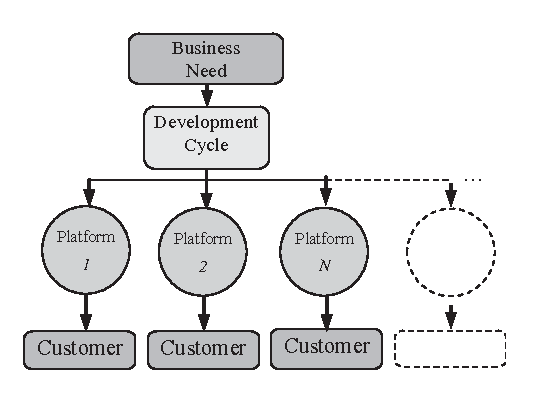
\includegraphics[width=10cm]{imagem/multiplataform-development.png}
    \caption*{Fonte: \cite{Corral2012}}
    \label{figura:multiplataform-development}
    \end{figure}
    
    
    A segunda alternativa para o desenvolvimento de \textit{apps} é a utilização de tecnologias voltadas à \textit{Web} \cite{S.ElKassas2015}. Posto que esta forma de desenvolvimento possibilita a redução de custos, tempo e esforço de desenvolvimento e manutenção do sistema, também exclui a necessidade de múltiplas equipes de desenvolvimento e possibilita a execução da aplicação em diferentes ambientes operacionais. A figura \ref{figura:multiplataform-development} demonstra como é a relação do ciclo de desenvolvimento e a distribuição destas aplicações aos usuários.
    
    \subsection{Aplicações nativas multiplataformas}
        \label{app_multiplataforma_nativa}
    
    São consideradas aplicações nativas multiplataformas, aquelas que a partir de um mesmo código fonte, podem ser instaladas e executadas com código nativo em diferentes sistemas operacionais. Em sua totalidade, este tipo de aplicação reúne todos os pontos positivos das aplicações nativas e hibrídas, explicitados nas subseções \ref{app_nativas} e \ref{app_hibridas}.
    
    \begin{figure}[h]
    \caption{Gráfico comparativo entre \textit{React Native}, \textit{Flutter} e \textit{Xamarin}}
    \centering % para centralizarmos a figura
    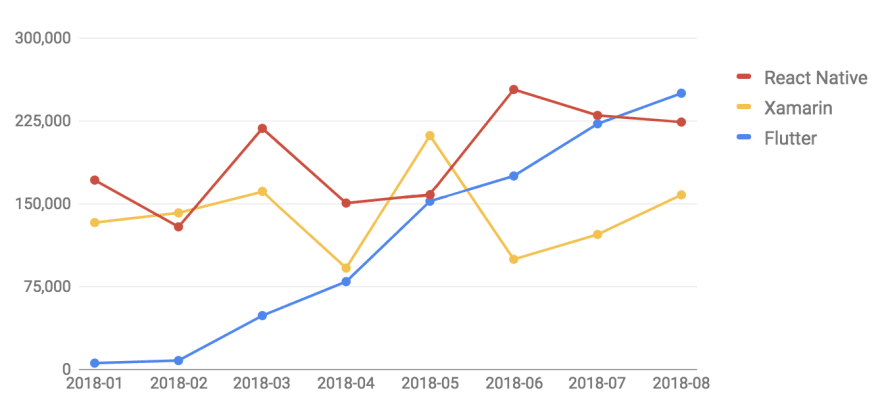
\includegraphics[width=12cm]{imagem/native-frameworks.jpg}
    \caption*{Fonte: \cite{Alferd2019}}
    \label{figura:native-frameworks}
    \end{figure}
    
    \textit{Flutter}, \textit{React Native} e \textit{Xamarin} são os três principais \textit{frameworks} que possibilitam esta abordagem. Na figura \ref{figura:native-frameworks} é apresentado um gráfico do crescimento da utilização destas ferramentas para o desenvolvimento \textit{mobile} ao longo dos anos, considerando a quantidade de aplicativos que utilizam estes \textit{frameworks}. Cada uma destas estruturas tem seus próprios prós e contras, o que dificulta muito realizar um comparativo que defina qual o melhor \textit{framework} a ser utilizado no desenvolvimento, tratando se de uma escolha pessoal e de fato alinhada à real necessidade de negócio na qual a aplicação será envolvida. Para o contexto deste trabalho e da aplicação desenvolvida será tratado com mais profundidade as concepções e particularidades mais relevantes sobre o \textit{React Native} e suas principais bibliotecas para o desenvolvimento.
    
    \section{Desenvolvimento \textit{mobile} nativo multiplataforma}

    De acordo com \citeonline{Corral2012}, aplicações móveis são desenvolvidas de forma dinâmica e lançadas no mercado em pequenos ciclos. Os produtos finais costumam ser de pequeno porte e comercializados a preços baixos. As equipes de desenvolvimento também tendem a ser pequenas. 
    
    Apesar do desenvolvimento \textit{mobile} nativo multiplataforma apresentar se diferentes em alguns pontos, as tradicionais e agéis metodologias e processos de desenvolvimento de software são totalmente aplicáveis neste contexto também, o que poderá diferenciar é apenas as características do produto final.
    
    Esta forma de desenvolvimento obteve um grande crescimento no mercado \textit{mobile} em razão da necessidade de muitas empresas obterem maior produtividade no processo de desenvolvimento junto a criação de aplicações robustas, performáticas e que sejam menos custosas à empresa. \textit{Facebook}, \textit{Instagram}, \textit{Airbnb}, \textit{Nubank} entre outras grandes empresas utilizam essas tecnologias em suas aplicações, com isso é perceptível o quanto essa metodologia de desenvolvimento é referência no mercado.
    
    Dentre as vantagens e diferenças já apresentadas sobre desenvolvimento nativo multiplataforma, pode-se destacar também a facilidade no desenvolvimento pelo fato da utilização de linguagens de programação mais comuns, o que evita a necessidade de um conhecimento aprofundado sobre uma linguagem específica e exclui a necessidade do estudo detalhado de cada plataforma operacional.

    \section{\textit{React Native}}
    \label{react_native}

  \citeonline{Inukollu2014} mostram a possibilidade de desenvolver de forma nativa usando \textit{React Native}, extensão do projeto \textit{React}, originalmente grafado como \textit{ReactJS}.
  
  \textit{React Native} é um \textit{framework} em \textit{JavaScript} para a criação de aplicativos \textit{mobile} reais e nativos para Android e iOS \cite{Eisenman2015}. Como citado, o \textit{React Native} utiliza em seu núcleo o \textit{React}, uma biblioteca em \textit{JavaScript} que se baseia na criação de interfaces através de JSX, uma extensão para o \textit{JavaScript} que possibilita escrever sintaxe XML em meio aos códigos da linguagem, sem qualquer semântica ou delimitação de \textit{tags}, possibilitando escrever a interface junto à lógica de programação.
    
    \subsection{Funcionamento}
    
    De acordo com as definições apresentadas na seção \ref{react_native}, este \textit{framework} grafado em \textit{ReactJS}, trabalha também com Virtual DOM para a renderização de suas interfaces. O DOM(\textit{Document Object Model}) é uma árvore composta de elementos gráficos em uma página e devido a sua estrutura, algumas mudanças destes elementos tendem a afetar em questões e performance e usabilidade das aplicações, porém o \textit{React} trabalha somente com a atualização do Virtual DOM de cada componente renderizado, buscando por alterações nos mesmos, comparando o estado do Virtual DOM com uma imagem do DOM feita antes das alterações e identificando o que realmente foi alterado para o incremento somente deste componente. É possível verificar este fluxo na figura \ref{figura:virtual-dom} abaixo.
    
    \clearpage
    
    \begin{figure}[h]
    \caption{Virtual DOM no React Native}
    \centering % para centralizarmos a figura
    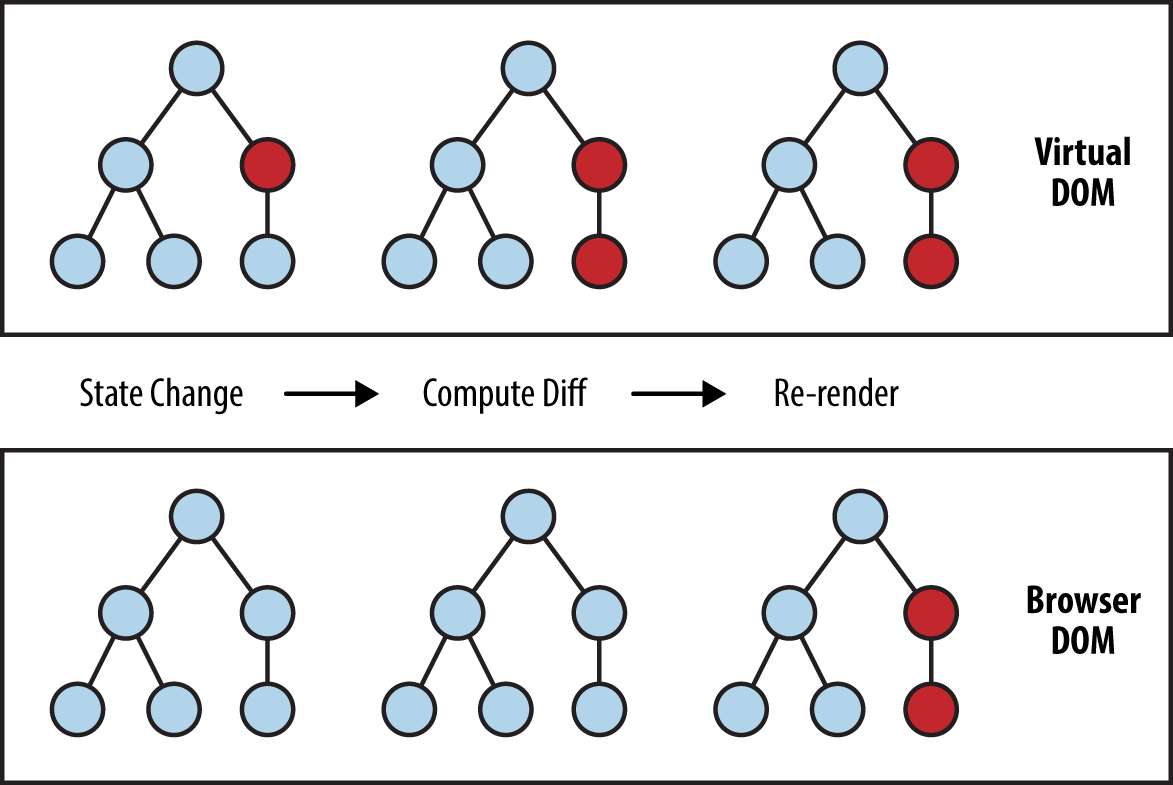
\includegraphics[width=10cm]{imagem/virtual-dom.png}
    \caption*{Fonte: \cite{Eisenman2016}}
    \label{figura:virtual-dom}
    \end{figure}
    
    Mesmo possuindo uma sintaxe semelhante à do \textit{ReactJS} por também utilizar o JSX, existe uma diferença na forma de renderização de seus elementos, conforme indicado na figura \ref{figura:react-native-component}. No React Native, os elementos são emulados de forma nativa, utilizando o \textit{JavaScript Core} que atua como uma ponte entre o JSX e as linguagens. Essa ponte abstrai uma camada de aplicação que possibilita executar API de renderização do \textit{Java}(Android) e do \textit{Objective-C}(iOS).
    
    \begin{figure}[h]
    \caption{Funcionamento da \textit{bridge} no React Native}
    \centering % para centralizarmos a figura
    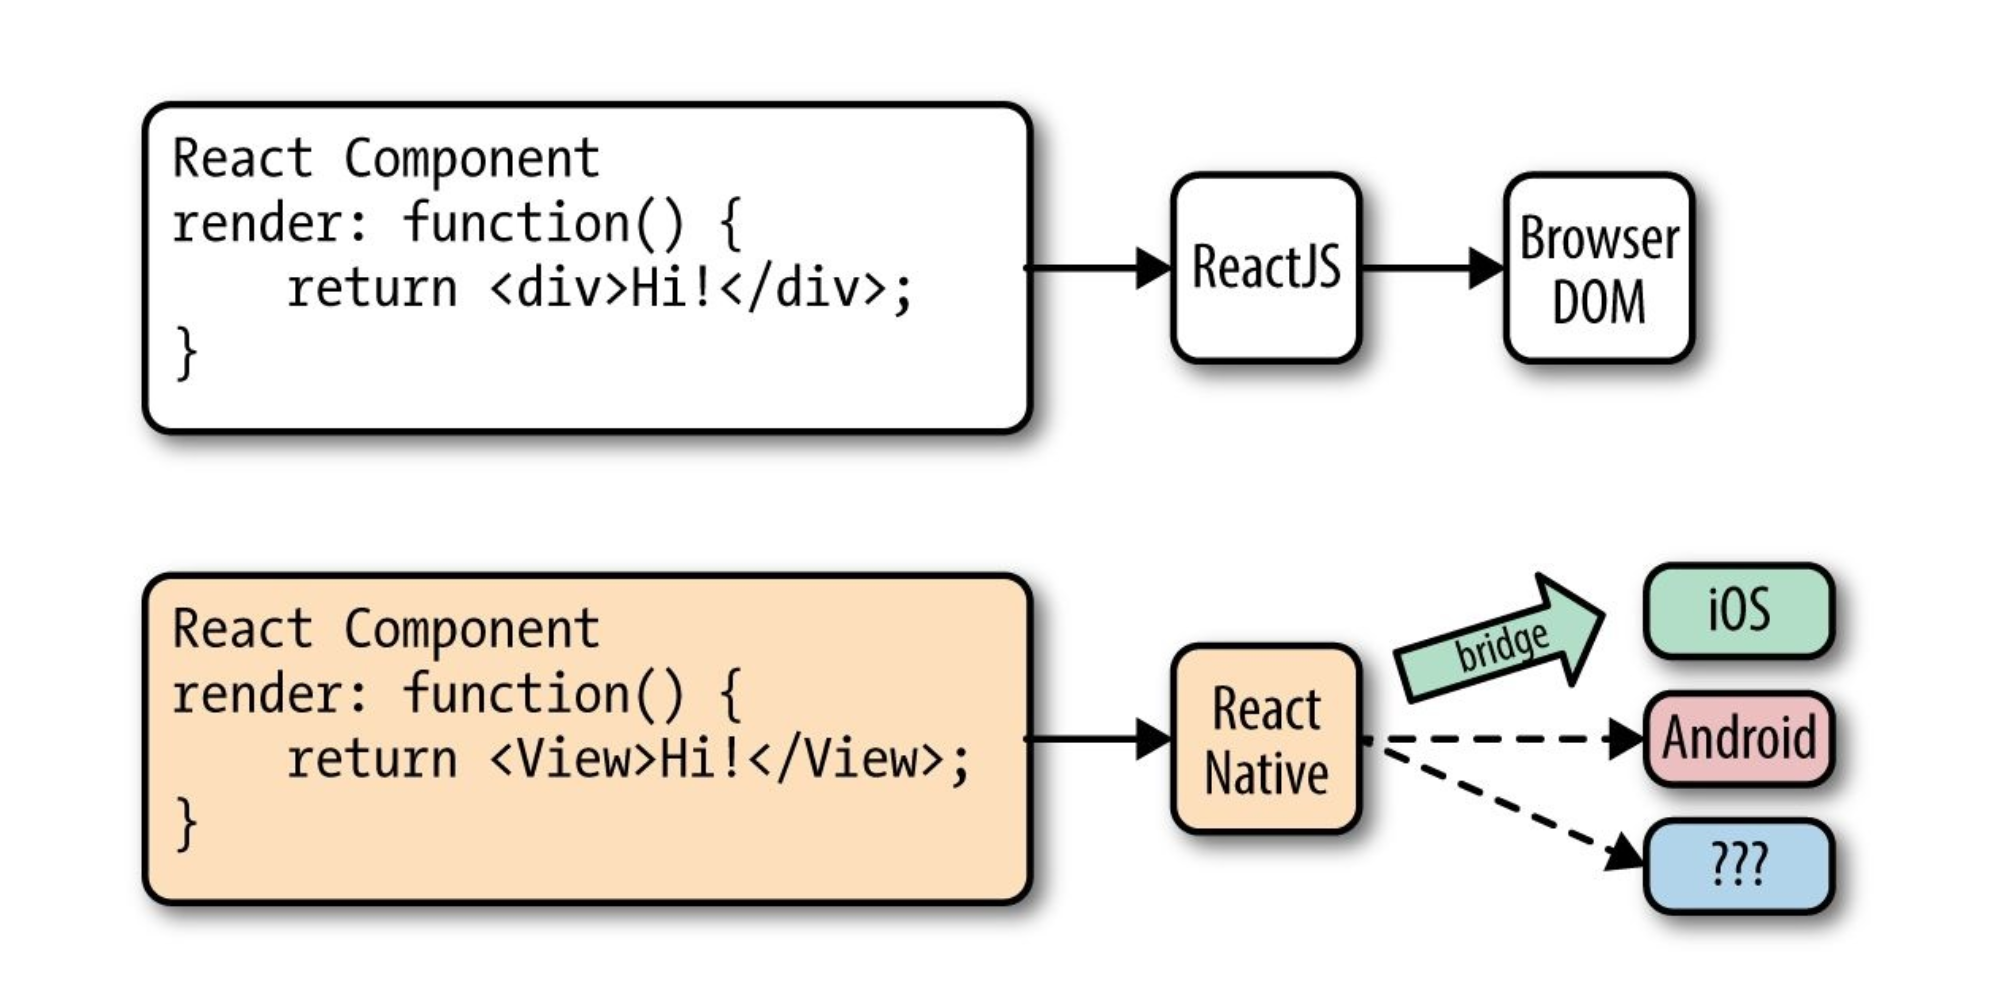
\includegraphics[width=10cm]{imagem/react-native-components.png}
    \caption*{Fonte: \cite{Eisenman2016}.}
    \label{figura:react-native-component}
    \end{figure}
    
    Este \textit{framework} possui três \textit{threads} para executar uma aplicação. A \textit{Shadow Queue}, onde o layout é manipulado; \textit{thread} principal, onde ocorre todo o processo de renderização da interface e a \textit{thread Javascript} onde os \textit{scripts} serão executados \cite{Danielsson998793}.
    
    A orquestração dos componentes nativos de sistema operacional é feita pela "ponte" ~que existe entre o núcleo nativo e o núcleo \textit{JavaScript}. De acordo  com \citeonline{Eisenman2016} Eisenman(2016,  p.  17), \begin{quote} [...] \textit{React  Native} invoca  as  APIs de renderização nativas em \textit{Objective-C} (para iOS) ou \textit{Java} (para Android), além disso ele transpila, minifica e otimiza um código feito em \textit{JavaScript} pelo seu próprio \textit{bundler} chamado \textit{Metro}. \end{quote}
    
    \subsection{Arquitetura}
    \label{react_native_mvp}
    
    Por sua clareza em termos de código, facilidade ao implementar testes automatizados e economia no tempo inicial da estruturação de um aplicativo, o MVP (\textit{Model-View-Presenter}) é um dos padrões mais adotados em aplicações \textit{React Native} e o seu fluxo de informações e troca de mensagens é representado abaixo na figura \ref{figura:react-native-mvp}.
    
    \begin{figure}[h]
    \caption{Fluxo de informações no MVP}
    \centering % para centralizarmos a figura
    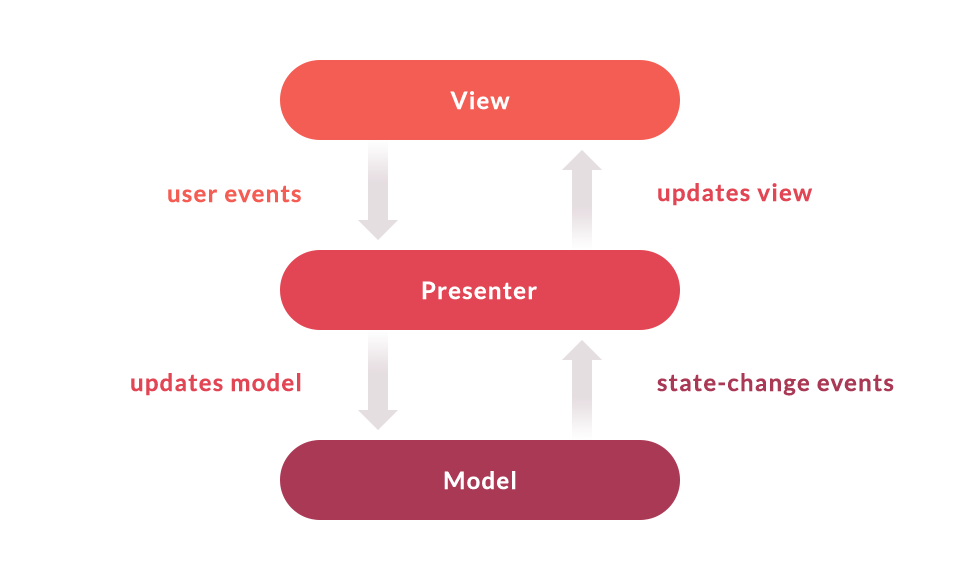
\includegraphics[width=12cm]{imagem/react-mvp.png}
    \caption*{Fonte: \cite{Teles2017}}
    \label{figura:react-native-mvp}
    \end{figure}
    
    O Model-View-Presenter é um padrão arquitetural derivado do MVC (\textit{Model-View-Controller}), a principal diferença é que no MVC o \textit{model} dispara atualizações ao \textit{view} sendo essas atualizações intermediadas pelo \textit{controller}, no MVP quem realiza essas intermediações é a camada \textit{presenter} sendo a principal responsabilidade deste componente, controlar o que será exibido ao \textit{view}, enquanto o \textit{view} é encarregado de organizar estes elementos para exibição ao usuário e o \textit{model} possui as mesmas atribuições que no padrão MVC.
    
    \section{Ferramentas e bibliotecas para o desenvolvimento em \textit{React Native}}
    \label{ferramentas-react-native}
    
    O objetivo desta seção é destacar e apresentar as definições das principais ferramentas e bibliotecas utilizadas no desenvolvimento do aplicativo para o laboratório de audiovisual e fotografia da PUC MINAS.
    
    \subsection{Expo}
    O Expo é uma ferramenta utilizada no desenvolvimento mobile com React Native que permite o fácil acesso às API’s nativas do dispositivo sem precisar instalar qualquer dependência ou alterar código nativo \cite{Fernandes2018}. Além disto, essa ferramenta possibilita o desenvolvimento sem a necessidade de instalar a SDK do Android e do XCode para Mac, possibilitando também a execução das versões de desenvolvimento do aplicativo em um dispositivo móvel que possui instalado o aplicativo Expo afim de testar e verificar o comportamento da aplicação na plataforma operacional.
    
    \subsection{React Navigation}
    É composto por alguns utilitários que criam uma estrutura de navegação em aplicativos \textit{React Native}. O React Navigation foi lançado em 2018 e é a biblioteca de navegação do \textit{React Native}, responsável por orquestrar todo o roteamento e navegação entre telas da aplicação de maneira simples e robusta.
    
    \subsection{Axios}
    Apesar de seu uso não ser exclusivamente do \textit{React Native}, o Axios é uma biblioteca que faz parte de todo o ecossistema \textit{JavaScript}, feita para realizar requisições HTTP baseando se no conceito de promises e é muito utilizada para consumir API's no intuito de buscar informações necessárias as aplicações.
    
    \subsection{ESLint}
    O ESLint é uma ferramenta utilizada para identificar e relatar padrões encontrados no código \textit{ECMAScript} / \textit{JavaScript}, com o objetivo de tornar-lo mais legível e consistente evitando possíveis problemas na codificação, antes de sua execução. Sua utilização é muito importante para padronizar espaçamentos e identações em todos os trechos de código da aplicação.
  
      
    \section{Aplicações correlatas}
    
    \subsection{GimmeBack}
    
    O GimmeBack é um aplicativo que permite aos usuários cadastrarem objetos que serão disponibilizados para empréstimo a terceiros e programarem a data para devolução do mesmo, além de contar com um sistema de alertas e notificações para recordar os usuários sobre os prazos.
    
    \begin{figure}[h]
    \caption{Tela de empréstimos ativos}
    \centering % para centralizarmos a figura
    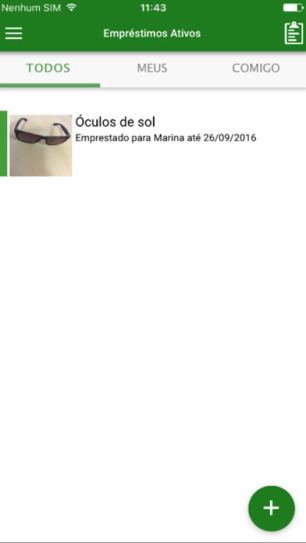
\includegraphics[width=8cm]{imagem/gimmeback-img.jpeg}
    \caption*{Fonte: \cite{MOBILE2016}}
    \label{figura:gimmeback}
    \end{figure}
    
    \subsection{Peerby}
    
    É um sistema que facilita o empréstimo de objetos entre pessoas que moram até 30 minutos de distância, funcional somente na Holanda, essa ferramenta tem como objetivo diminuir compras de coisas que são necessárias em poucos momentos, criando uma ideia mais sustentável de consumo. Em funcionalidades, o solicitante cadastra o objeto que está procurando, enquanto os demais usuários que possuírem aquele item, entram na solicitação e alertam o solicitante sobre a disponibilidade de realizar o empréstimo, um fluxo inverso se comparado ao GimmeBack e o aplicativo do laboratório.
    
    \begin{figure}[h]
    \caption{Tela de vizinhos próximos}
    \centering % para centralizarmos a figura
    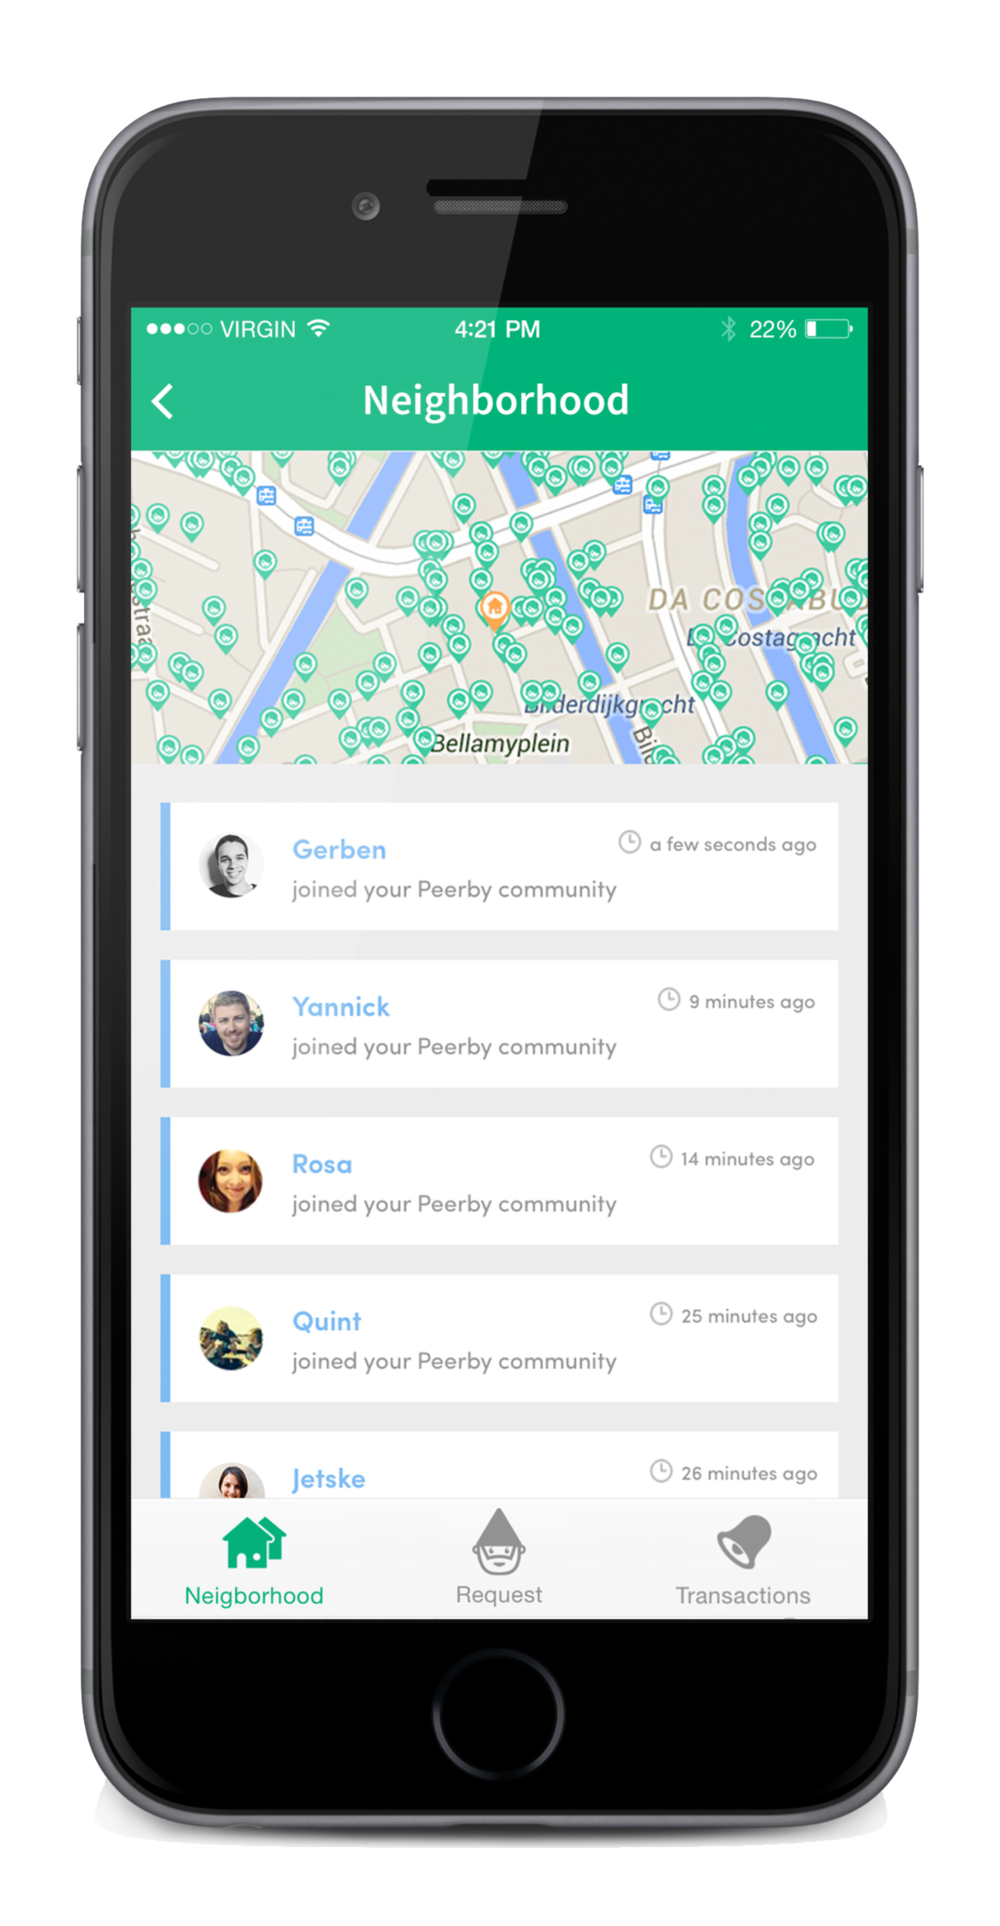
\includegraphics[width=8cm]{imagem/peerby-img.png}
    \caption*{Fonte: \cite{PEERBY2014}}
    \label{figura:peerby}
    \end{figure}
    
    \subsection{Tem açucar?}
    
    Seguindo a mesma linha do Peerby, o aplicativo Tem açucar? foi criado com o objetivo de promover o compartilhamento de objetos com vizinhos, de modo sustentável e que promova uma boa relação entre os mesmos. Portanto é possível buscar por objetos a serem emprestados pela plataforma, avaliar a experiência de empréstimo e ter acesso a esses objetos de forma mais simples e segura.
    
    \begin{figure}[h]
    \caption{Tela de solicitação}
    \centering % para centralizarmos a figura
    \includegraphics[width=8cm]{imagem/temaçucar-img.jpg}
    \caption*{Fonte: \cite{NATALIA2020}}
    \label{figura:comparative-board}
    \end{figure}
    
    \subsection{Comparativo}
    
    Além do quadro comparativo abaixo, é importante destacar o propósito e o público alvo de cada aplicativo citado anteriormente. Começando pelo GimmeBack que tem o objetivo de tornar se uma comunidade de compartilhamento de objetos sem com que as pessoas tenham dificuldades em emprestar e receber de volta seus itens, atualmente o aplicativo é utilizado até por algumas bibliotecas escolares para organizar melhor o empréstimo de livros a alunos. Em seguida, apesar de ainda não funcionar no Brasil, o aplicativo Peerby busca influenciar boas práticas conectando vizinhos ou pessoas de um mesmo bairro para que os mesmo compartilhem seus pertences entre si, socializando as ideias e necessidades cotidianas e o aplicativo Tem Açucar? propõe a ideia de uma rede social de vizinhos que facilite a comunicação, colaboração e troca de gentilezas nas vizinhanças. Em contra ponto, o aplicativo desenvolvido para o laboratório de audiovisual e fotografia da PUC MINAS, apesar de compartilhar algumas semelhanças em termos de funcionalidade e ideia central, tem seu público alvo focado nos alunos da universidade com um nicho pré definido de objetos/equipamentos que irão compor os cenários dos empréstimos.
    
    \begin{figure}[h]
    \caption{Quadro comparativo}
    \centering % para centralizarmos a figura
    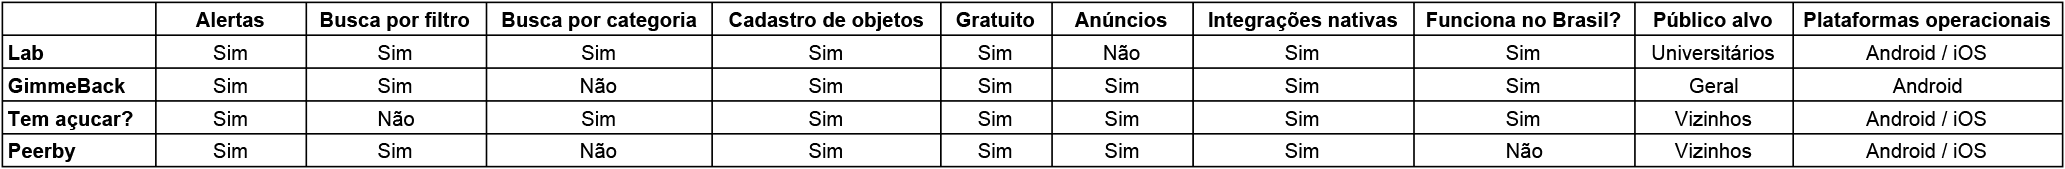
\includegraphics[width=16cm]{imagem/quadro-comparativo.png}
    \caption*{Fonte: Autor}
    \label{figura:comparative-board}
    \end{figure}

% Nome do capítulo
\chapter{METODOLOGIA}
% Label para referenciar
\label{cap3}

% Diminuir espaçamento entre título e texto
\vspace{-1.9cm}

% Texto do capítulo

    Para que o desenvolvimento do trabalho esteja alinhado as necessidades do laboratório de audiovisual e fotografia seria preciso, em um primeiro momento, elicitar todos os requisitos arquiteturais (funcionais e não funcionais) de maneira que o entedimento do escopo do projeto fique claro. Os requisitos são descritos textualmente para identificar as funcionalidades e características que a aplicação deve possuir para conseguir realizar as ações que, em conjunto, solucionam o problema exposto, sendo assim, tem-se uma visão de alto nível do projeto, o que torna sua interpretação fácil a todos os envolvidos.
    
    Com a definição do escopo do projeto e dos requisitos, seria criado um protótipo da parte visual que contemple as principais interfaces do aplicativo e seus respectivos componentes, além de elaborar diagramas de classe e de componentes que retratam como o software irá se comportar de maneira oculta e como esses componentes irão persistir dados, a estrutura lógica do banco de dados e qual tipologia de dados seria mais adequeada ao problema que este trabalho irá resolver. Dado a criação destes diagramas que apresentam a arquitetura de funcionamento do software é possível compreender como será o fluxo de comunicação do aplicativo e a apresentação das informações pertinentes aos usuários durante o uso.
    
    Conforme apresentado na figura \ref{figura:lab-architecture} é possível visualizar a arquitetura da aplicação \textit{mobile}, o fluxo de comunicação entre os componentes e os padrões de projeto adotados para desenvolver esta solução, na API Rest desenvolvida para suportar as funcionalidades do aplicativo e suas operações no banco de dados, encontra se o padrão MVC, semelhante ao padrão MVP, apresentado na subseção \ref{react_native_mvp} e que foi aplicado no aplicativo em \textit{React Native}.
    
    \clearpage
    
    \begin{figure}[h]
    \caption{Arquitetura do aplicativo}
    \centering % para centralizarmos a figura
    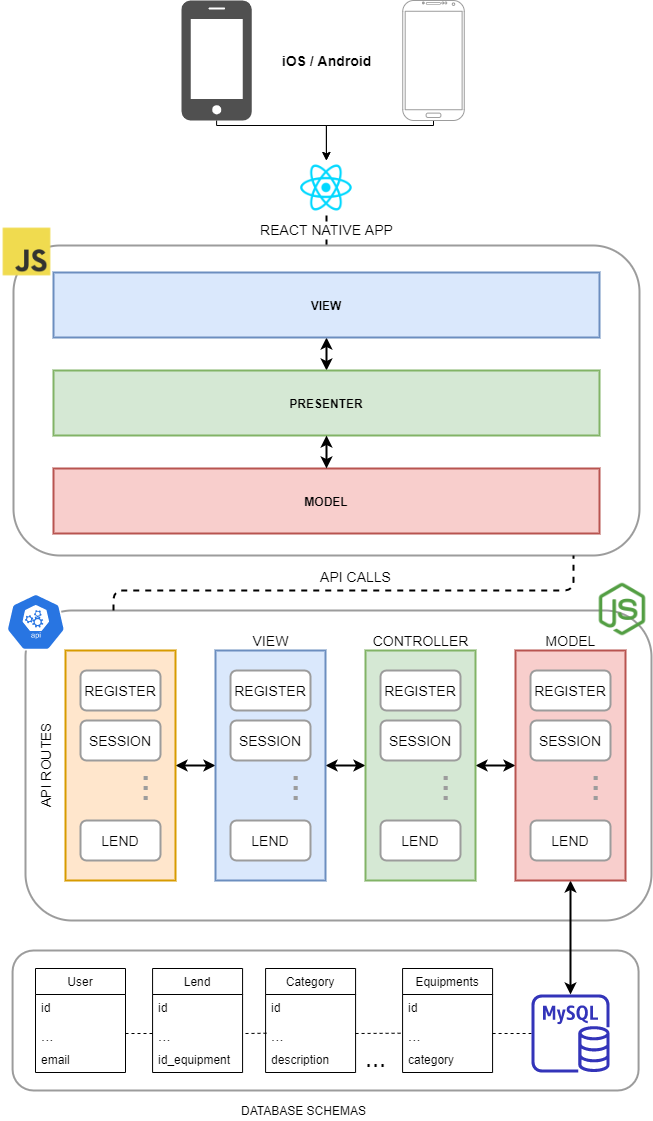
\includegraphics[width=12cm]{imagem/jubilant-octo-lab.png}
    \caption*{Fonte: Autor}
    \label{figura:lab-architecture}
    \end{figure}
    
    \clearpage
    
    Após essas definições de arquitetura, citadas no paragráfo anterior, serão selecionadas as ferramentas e as principais bibliotecas disponibilizadas pelo JavaScript para compor o processo de desenvolvimento e a codificação do aplicativo, junto à escolha da estrutura de hierárquica de diretórios, configuração do ambiente de desenvolvimento e ambiente para os testes.
    
    A penúltima etapa consiste no desenvolvimento do aplicativo em si, considerando todos requisitos pré definidos e seguindo as especificações de interface elaborada na etapa de prototipagem e a escrita dos testes unitários e de integração para validar o comportamento do sistema perante o uso de suas funcionalidades, simulando objetos/usuários reais com metódos disponibilizados pelas bibliotecas que estão em uso na aplicação.
    
    E por fim, a implantação e disponibilização do aplicativo em Android e iOS, para alguns alunos e monitores da Universidade para analisar como o sistema se comporta em situações reais de empréstimo de equipamentos do laboratório. %Segue abaixo na tabela \ref{table:cronograma-tcc} o cronograma detalhado para o desenvolvimento do trabalho.
    
  %  \begin{table}[htb]
  %  \caption{Cronograma}
  %  \centering % para centralizarmos a figura
  %  \includegraphics[width=16cm]{imagem/cronograma-tcc.png}
  %  \caption*{Fonte: Autor}
  %  \label{table:cronograma-tcc}
  %  \end{table}


% Nome do capítulo
\chapter{DESENVOLVIMENTO}
% Label para referenciar
\label{cap4}

% Diminuir espaçamento entre título e texto
\vspace{-1.9cm}

% Texto do capítulo
% Nome do capítulo
\chapter{CONCLUSÃO}
% Label para referenciar
\label{cap5}

% Diminuir espaçamento entre título e texto
\vspace{-1.9cm}

% Texto do capítulo

% PÓS-TEXTUAIS %%
% Bibliografia no arquivo 'Dissertacao.bib'
% Alterar o título das referências para somente 'Referências'
%\renewcommand{\bibname}{Referências}
\renewcommand{\bibname}{Referências}
\bibliographystyle{abnt-alf}
\bibliography{Dissertacao}
%\bibliographystyle{abnt-alf}


% Para forçar que os apêndices e anexos comecem no anverso
%\setboolean{@openright}{true}

%\apendice
%\begin{apendice}
%%------------------------------------------------------------------------------------------------------------------------------------------------------
% Reiniciar numeração das figuras que aparecem no apêndice
\setcounter{figure}{0}

\chapter{Primeiro apêndice}
\label{apend:codigoMpe}

% Para diminuir espaçamento entre o título e o texto
\vspace{-1.9cm}

%\end{apendice}

%\anexo
%% Nome do Anexo
\chapter{Primeiro Anexo}

% Para diminuir espa�amento entre o t�tulo e o texto
\vspace{-1.9cm}

% Texto

\end{document}